\documentclass[10pt, twocolumn]{article}

\usepackage[margin=0.75in]{geometry}
\usepackage{amsmath,amsthm,amssymb}
\usepackage{booktabs}
\usepackage{xcolor}
\usepackage{cancel}
\usepackage{graphicx}
\usepackage{lipsum}
\usepackage{changepage}
\usepackage{circuitikz}
\usepackage{pgfplots}
\usepackage{physics}
\usepackage{hyperref}
\usepackage[uncertainty-mode = separate, separate-uncertainty-units = single]{siunitx}
\usepackage{fontspec}
\usepackage{relsize}
\usepackage{todonotes}
\usepackage[breakable]{tcolorbox}
\usepackage[inline]{enumitem}
\patchcmd{\thebibliography}{\section*{\refname}}{}{}{}

\pgfplotsset{compat=newest}
\usetikzlibrary{arrows}
\usetikzlibrary{calc}
\usetikzlibrary{patterns}

\definecolor{incolor}{HTML}{303F9F}
\definecolor{outcolor}{HTML}{D84315}
\definecolor{cellborder}{HTML}{CFCFCF}
\definecolor{cellbackground}{HTML}{F7F7F7}
\newcommand{\ui}{\hat{i}}
\newcommand{\uj}{\hat{j}}
\newcommand{\uk}{\hat{k}}
\newcommand{\ux}{\hat{x}}
\newcommand{\uy}{\hat{y}}
\newcommand{\uz}{\hat{z}}
\newcommand{\primed}[1]{#1^\prime}
\usetikzlibrary{positioning, fit, calc}
\pgfdeclarelayer{background}  
\pgfsetlayers{background,main}
\AtBeginDocument{\RenewCommandCopy\qty\SI}
\definecolor{LightGray}{gray}{0.9}

\makeatletter
\newcommand{\boxspacing}{\kern\kvtcb@left@rule\kern\kvtcb@boxsep}
\makeatother
\newcommand{\prompt}[4]{
    \ttfamily\llap{{\color{#2}[#3]:\hspace{3pt}#4}}\vspace{-\baselineskip}
}

\newcommand{\highlight}[1]{\colorbox{yellow}{$\displaystyle #1$}}

\newcommand{\ti}[1]{\widetilde{#1}}

% Jeremy TODO if needed
% \newfontface{\Kaufmann}{Kaufmann}
% \DeclareTextFontCommand{\kf}{\Kaufmann}
% \newcommand{\scriptr}{\fontsize{12pt}{12pt}\kf{r}}

% \newfontface{\KaufmannB}{Kaufmann Bold}
% \DeclareTextFontCommand{\kfb}{\KaufmannB}
% \newcommand{\bscriptr}{\fontsize{12pt}{12pt}\kfb{r}}

\newcommand{\bv}[1]{\mathbf{#1}}

\title{Physics 3200Y: Lab 2}
\author{Jeremy Favro (0805980), Bryan Roberts (0691165), Melodie Johnston (??)
 \\\emph{Department of Physics \& Astronomy}\\ Trent University, Peterborough, ON, Canada}
\date{\today}

\begin{document}
\maketitle
\begin{abstract}
    
\end{abstract}
Blah balh
\section{Introduction}
This lab seeks to develop techniques to calculate capacitance of a constructed capacitor at varying frequencies and configurations. Additionally, through relationships derived in this report, the properties of the dielectric used in the construction of the capacitor are determined. Several new-to-the-authors techniques were developed through the course of this lab such as Fourier transforms.
\section{Theory}
\todo{Maybe squeeze a derivation of the expression for phase in here somewhere. See 2b?}
\subsection{Sawyer-Tower Circuit}
The Sawyer-Tower circuit was used to facilitate data collection on the constructed capacitor. \todo{Do the derivation for the capacitances. Maybe some explanation of why ST circ is useful. See assn. 5.}
\begin{figure}[h]
    \centering
    \begin{circuitikz}
  \draw (0,0) to[sV=$V$] ++(0,-2) to[capacitor, l=$C_s$, voltage dir=RP, v=$V_r$] ++(0,-2) coordinate(J1) to[capacitor, l=$C_r$] 
  ++(0,-2) coordinate(J2) node[ground]{} ++(0,-1)
  (J1) -- ++(1.75,0) to[resistor, l=$R_{osc}$] ++(0,-2) -| (J2)
  ;
\end{circuitikz}
    \caption{The Sawyer-Tower circuit. $C_s$ is the sample capacitor whose properties are to be investigated, $C_r$ is a reference capacitor of known parameters. $R_{osc}$ is \textbf{something?? idk what}}
    \label{circuit:sawyer-tower}
\end{figure}
\subsection{Complex Capacitance}
\subsection{Fourier Transform}
Note that we just used numpy's r(eal)fft implementation. We may still want to sketch out the tutorial we did on it though.
\section{Methods}
\subsection{Capacitor Construction}
\begin{figure}[h]
    \centering
    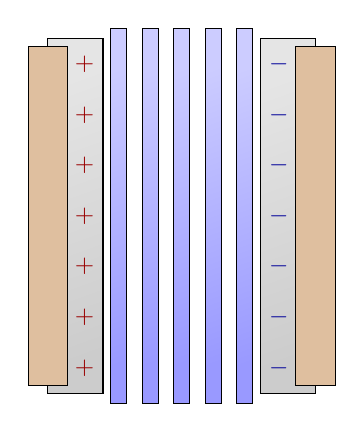
\begin{tikzpicture}
  \tikzstyle{dielectric}=[top color=blue!20,bottom color=blue!40,shading angle=20]
  \tikzstyle{foil}=[top color=gray!20,bottom color=gray!40,shading angle=20]
  \colorlet{pluscol}{red!60!black}
  \colorlet{minuscol}{blue!60!black}

  \def\H{4.5}
  \def\W{2.0}
  \def\w{0.7}
  \def\a{0.15*\W}
  \def\NE{6}
  \def\NQ{7}
  
  % DIELECTRIC
  \foreach \i [evaluate={\x=(\i-0.75)*\W/5}] in {1,...,5}{
      \draw[dielectric]
      (\x,-0.03*\H) rectangle (\x+0.1*\W,1.03*\H);
    }

  % PLATES
  \draw[foil]
  (0,0) rectangle++ (-\w,\H);
  \draw[fill=brown!50]
  (-0.45,0.1) rectangle ++(-\w+0.2,\H-0.2);

  \draw[foil]
  (\W,0) rectangle++ (\w,\H);
  \draw[fill=brown!50]
  (\W+0.45,0.1) rectangle ++(\w-0.2,\H-0.2);
  \foreach \i [evaluate={\y=(\i-0.5)*\H/\NQ;}] in {1,...,\NQ}{
      \node[pluscol,scale=0.9] at (-\w/3,\y) {$+$};
      \node[minuscol,scale=0.9] at (\W+\w/3,\y) {$-$};
    }
\end{tikzpicture}
    \caption{A cartoon of the constructed capacitor. The dielectric sheets (in blue) are represented with exaggerated spacing.}
    \label{illustration:homemade-cap}
\end{figure}
\subsection{Data Collection}
\section{Results}
The capacitance of the constructed capacitor was successfully determined using data collected from the Sawyer-Tower circuit and numpy's rfft. \todo{cite!} From this the dielectric ``constant'' was calculated using equation \todo{derive and cite} and found to vary not insignificantly with frequency. This is consistent with real-world data collected on the dielectric \emph{functions} $\epsilon(\omega)$ of many materials, even those designed to have similar dielectric/optical properties over large frequency ranges. 
\subsection{Capacitances \& Resistances}
\todo{Legends}
\begin{figure}[h]
    \centering
\begin{tikzpicture}
  \begin{axis}[
      xmode=log,
      xlabel={Peak FFT Frequency (Hz)},
      ylabel={$C_s\,(\unit{\farad})$}
    ]
    \addplot table [x=freq (Hz), y=C_s (nF), col sep=comma] {0.17cm processed.csv};
    \addplot table [x=freq (Hz), y=C_s (nF), col sep=comma] {0.3cm processed.csv};
    \addplot[mark=triangle*, brown] table [x=freq (Hz), y=C_s (nF), col sep=comma] {0.49cm processed.csv};
  \end{axis}
\end{tikzpicture}
    \caption{Recovered capacitances vs. recovered FFT peak frequencies}
    \label{fig:caps}
\end{figure}

\begin{figure}[h]
    \centering
\begin{tikzpicture}
  \begin{axis}[
      xmode=log,
      xlabel={Peak FFT Frequency (Hz)},
      ylabel={$R\,(\unit{\ohm})$}
    ]
    \addplot table [x=freq (Hz), y=R, col sep=comma] {0.17cm processed.csv};
    \addplot table [x=freq (Hz), y=R, col sep=comma] {0.3cm processed.csv};
    \addplot[mark=triangle*, brown] table [x=freq (Hz), y=R, col sep=comma] {0.49cm processed.csv};
  \end{axis}s
\end{tikzpicture}
    \caption{Recovered resistances vs. recovered FFT peak frequencies}
    \label{fig:res}
\end{figure}

\begin{figure}[h]
    \centering
\begin{tikzpicture}
  \begin{axis}[
      xmode=log,
      xlabel={Peak FFT Frequency (Hz)},
      ylabel={$\epsilon/\epsilon_0$}
    ]
    \addplot table [x=freq (Hz), y=eps (/e_0), col sep=comma] {0.17cm processed.csv};
    \addplot table [x=freq (Hz), y=eps (/e_0), col sep=comma] {0.3cm processed.csv};
    \addplot[mark=triangle*, brown] table [x=freq (Hz), y=eps (/e_0), col sep=comma] {0.49cm processed.csv};
  \end{axis}s
\end{tikzpicture}
    \caption{$\epsilon/\epsilon_0$ vs. recovered FFT peak frequencies}
    \label{fig:eps}
\end{figure}
\subsection{Dielectric Function}
The dielectric function was successfully calculated using the \todo{ref} derived formula. As can be seen in $\ref{fig:eps}$ is sits between 2.4 and 2.8 (in units of $\epsilon_0$) which is a reasonable range for common plastics which generally sit between 2 and 5 \cite{dielectric-plastics}
\clearpage
\subsection{Fourier Transform}
A Fourier Transform was successfully applied to the gathered data using Numpy's builtin \texttt{numpy.fft.rfft} function. As discussed in section 2.3 the Fourier Transforms are used to calculate \todo{Make sure it is discussed} the capacitance and thereby dielectric function. The actual effect of the transform is not very evident there, so it is discussed in more detail here.
\begin{figure*}[t]
    \centering
    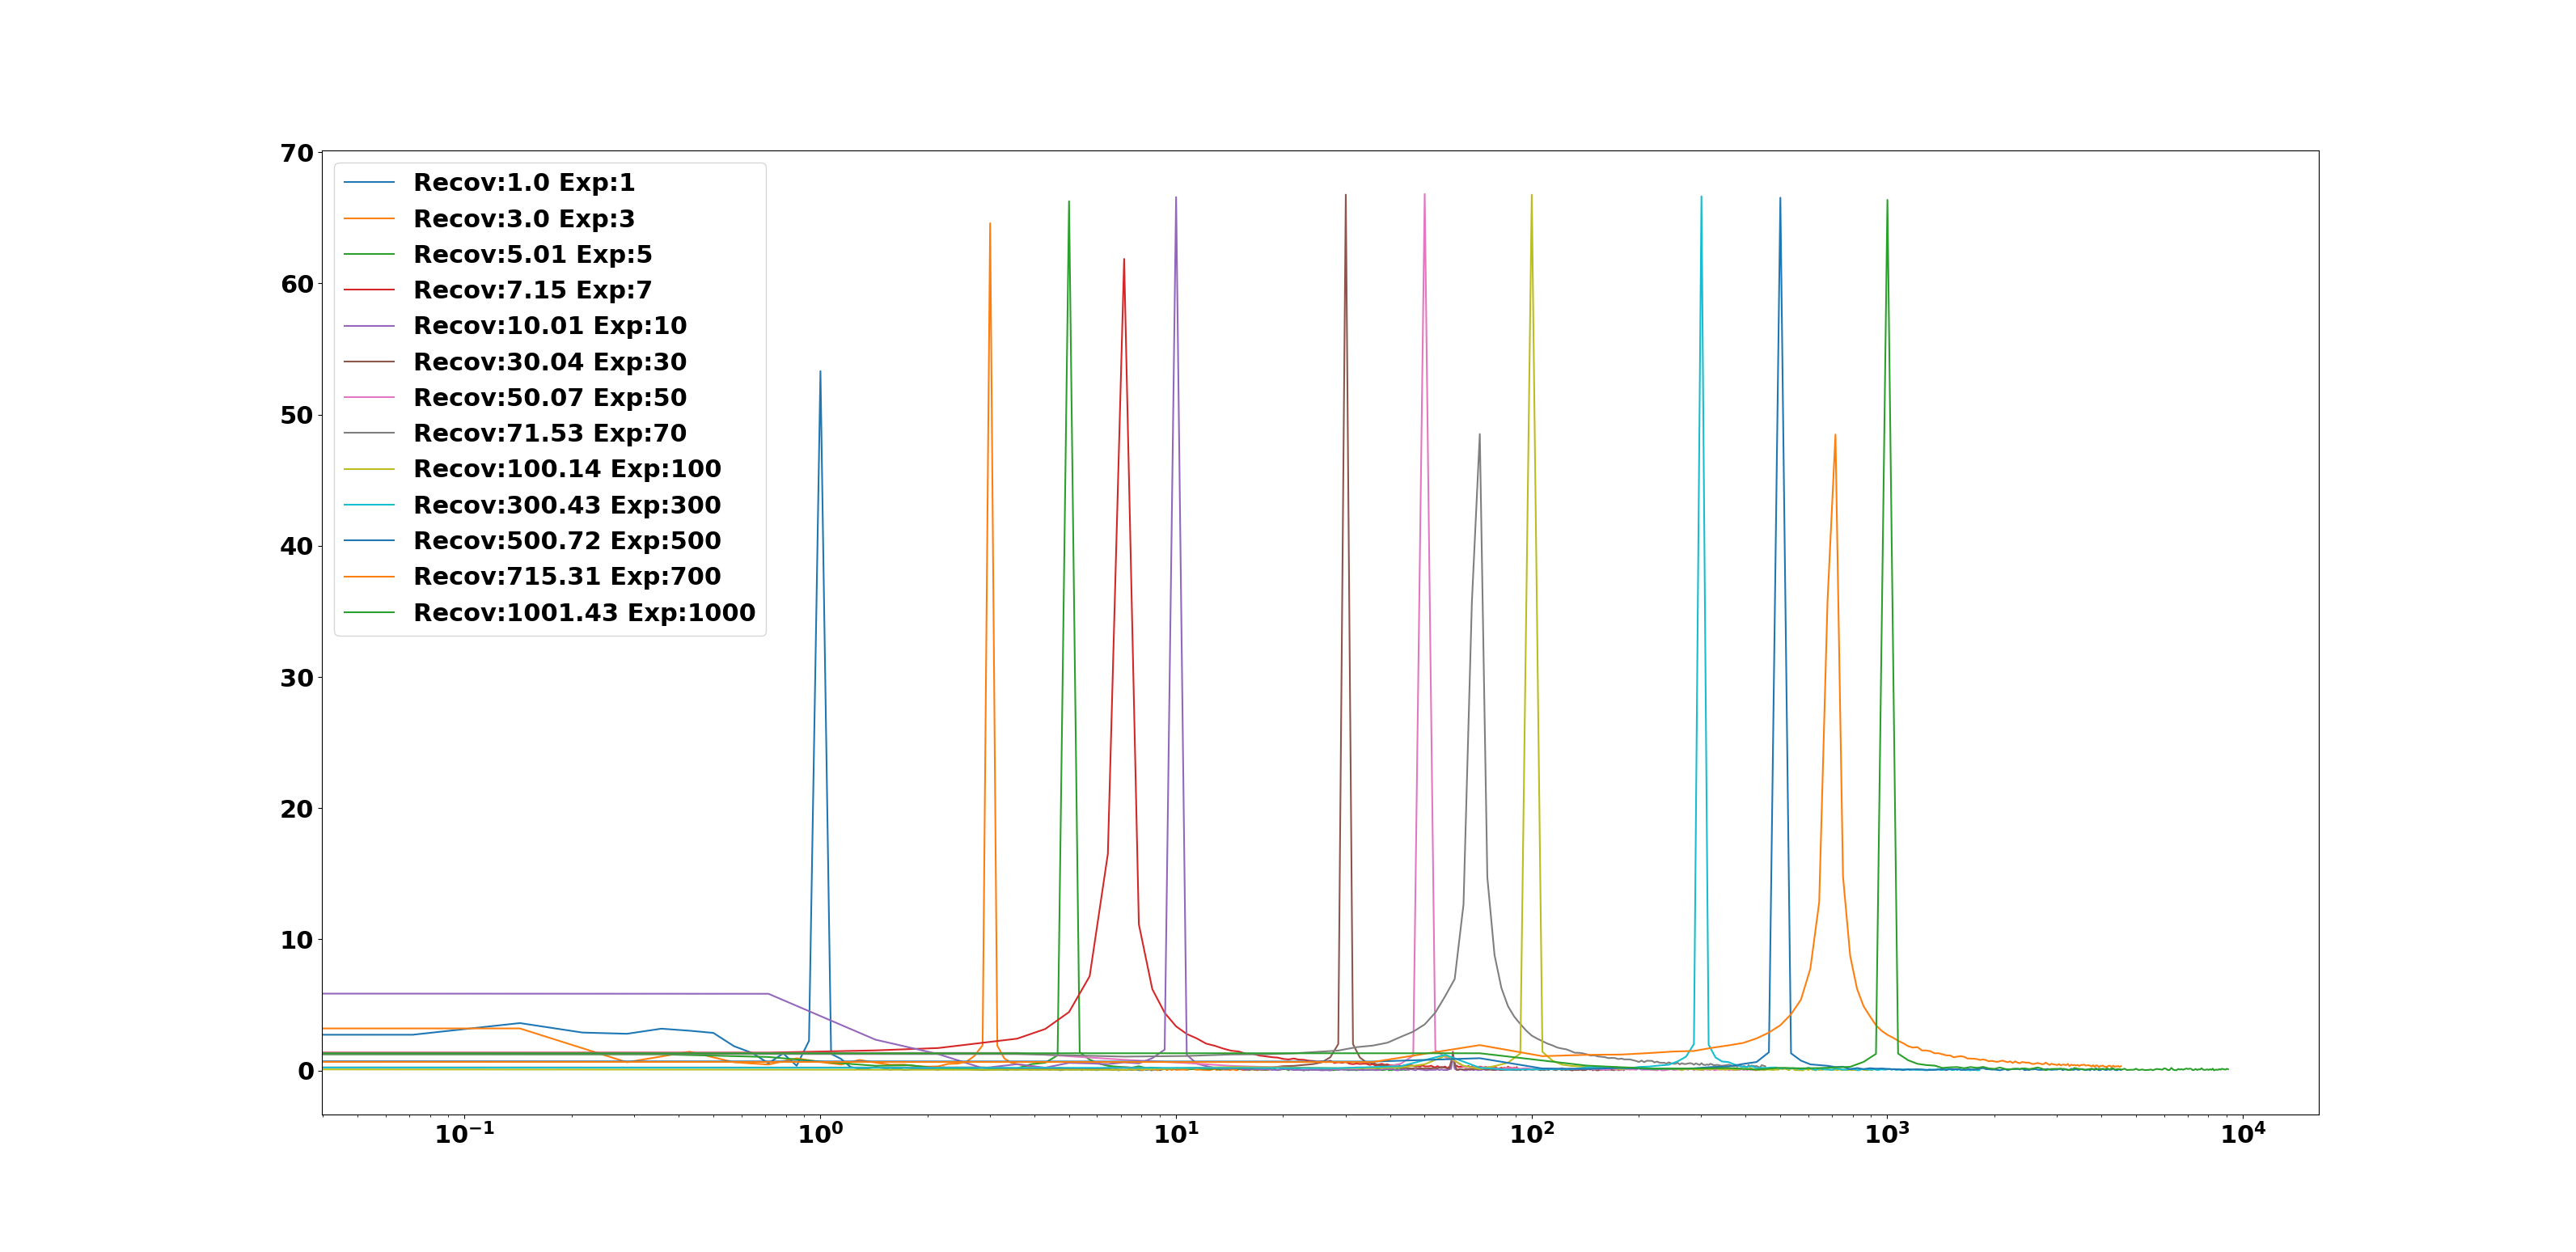
\includegraphics[width=\textwidth]{fft.png}
    \caption{FFT coefficients vs. Frequency from $V_r$.}
    \label{fig:fft}
\end{figure*}

v\begin{figure*}[t]
    \centering
    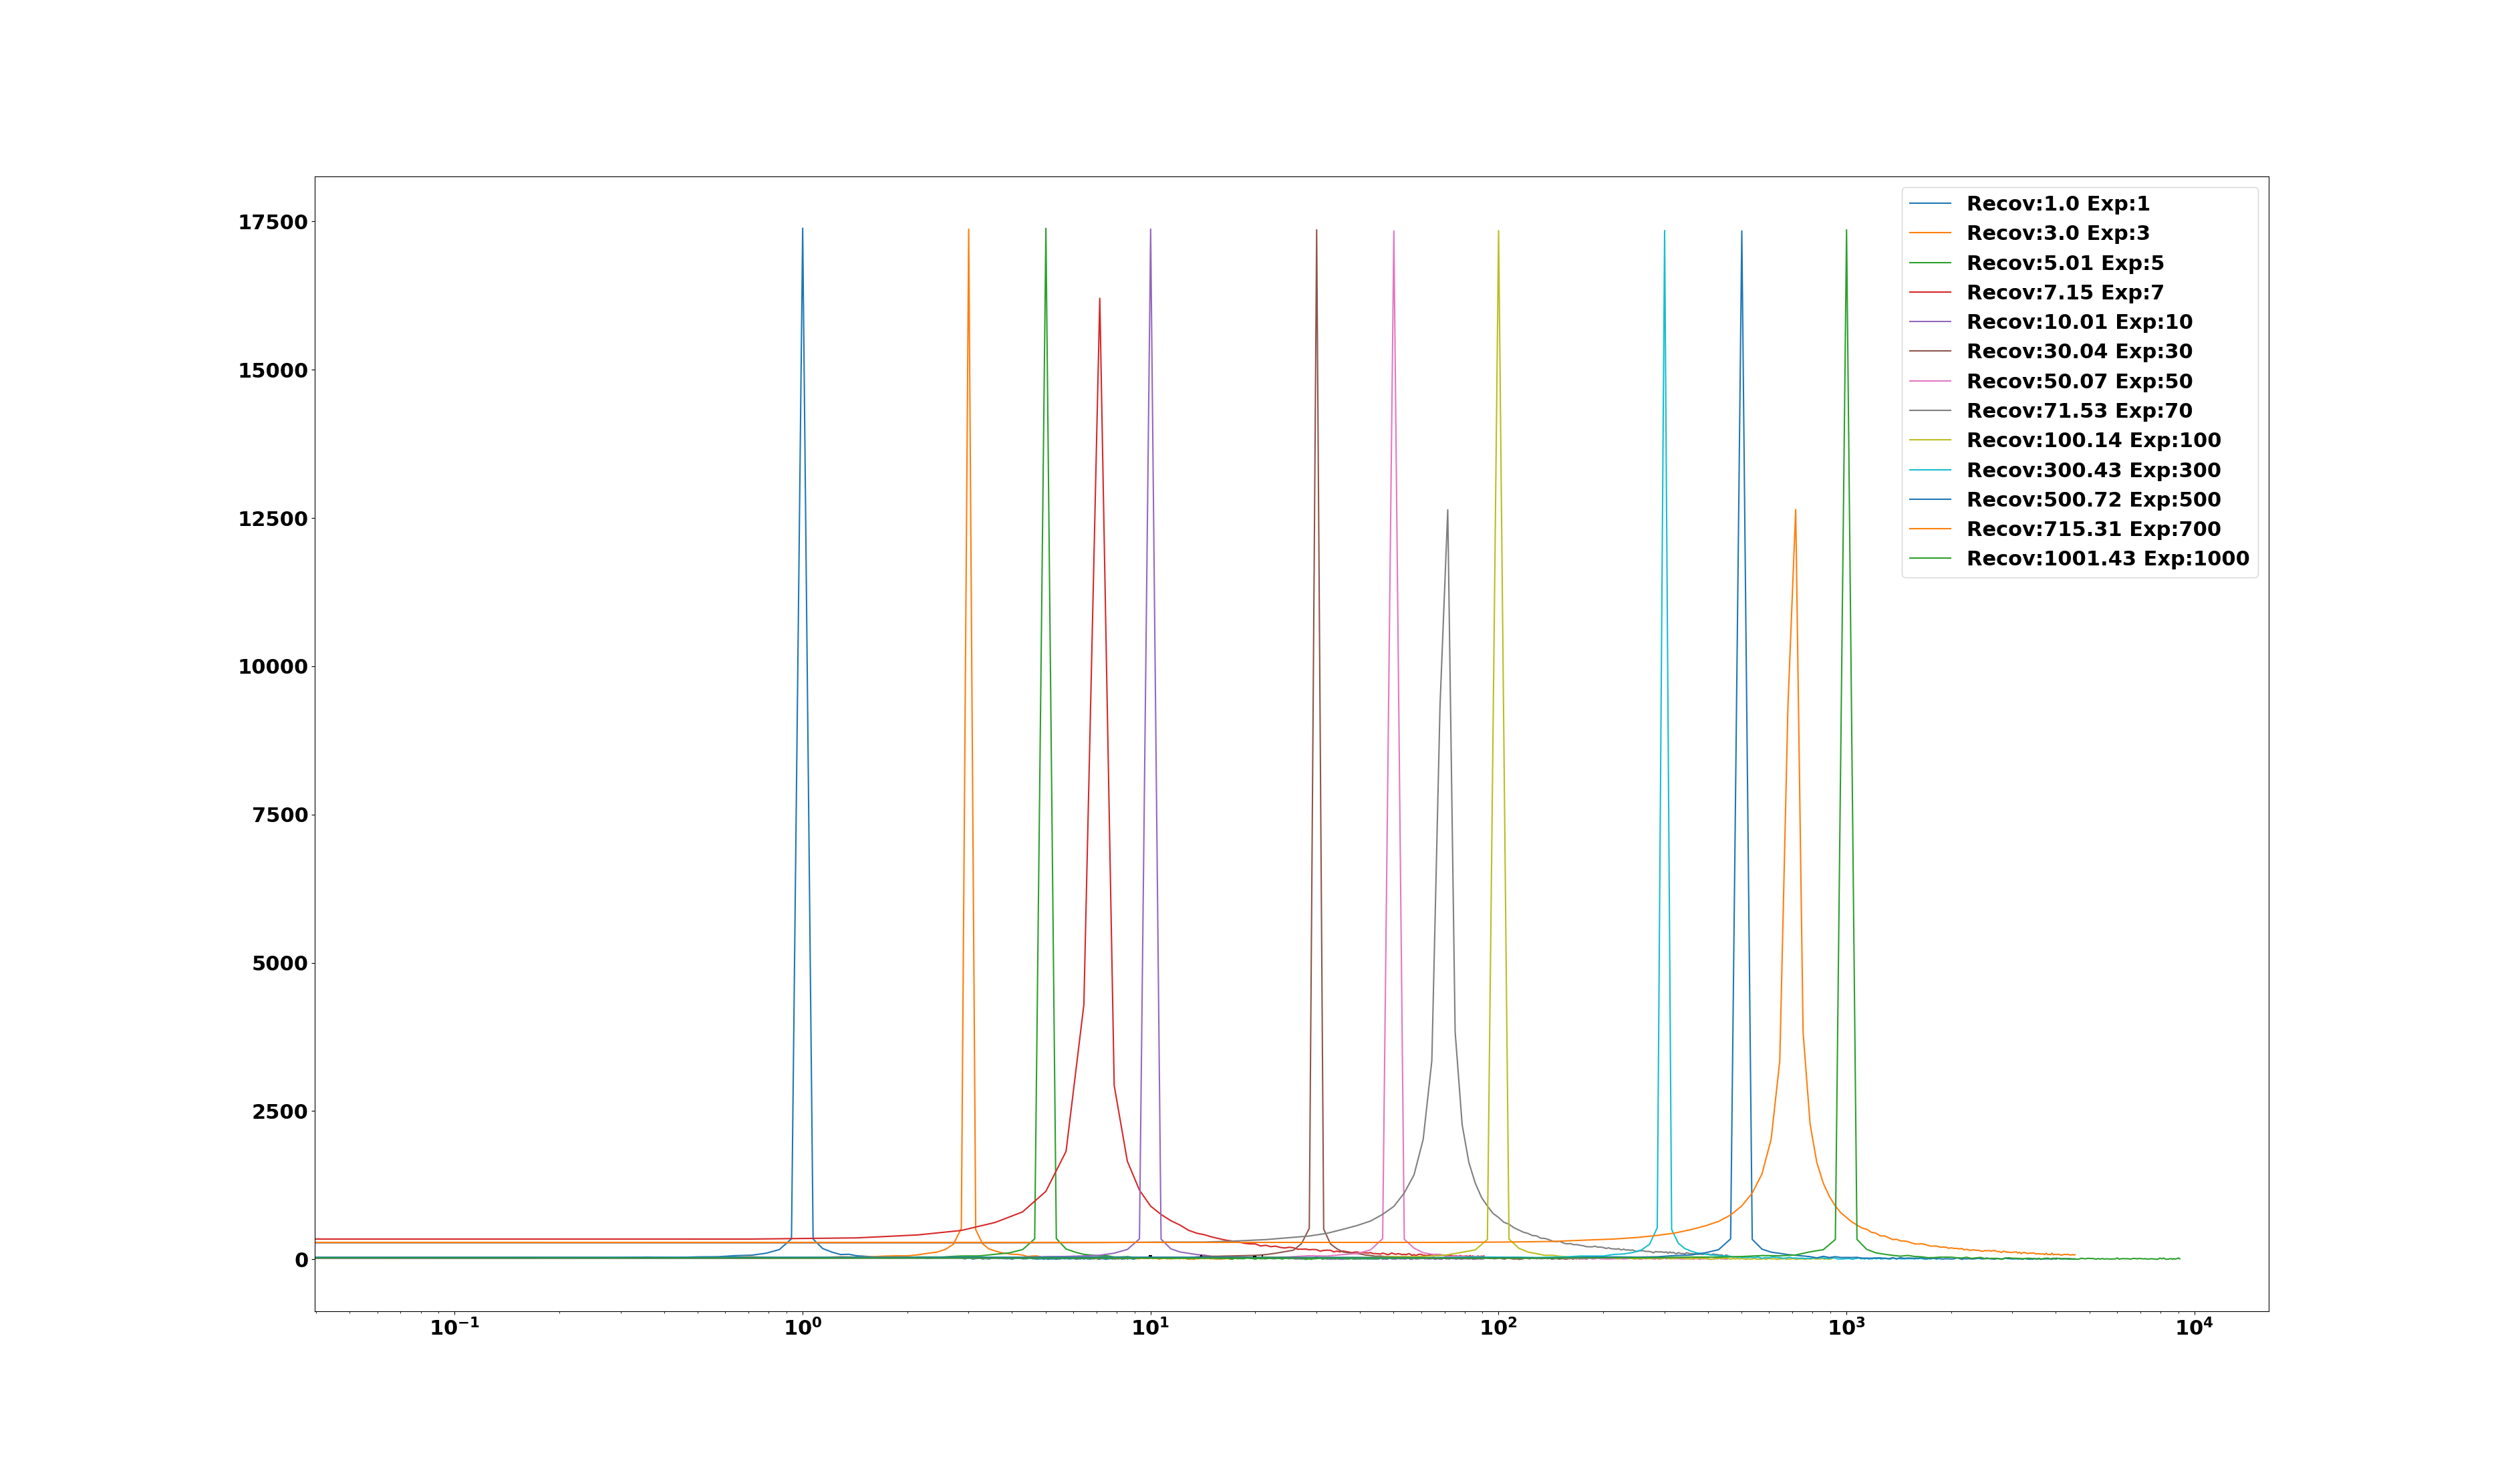
\includegraphics[width=\textwidth]{fft1.png}
    \caption{FFT coefficients vs. Frequency from $V$, the signal directly from the function generator.}
    \label{fig:fft1}
\end{figure*}
As seen in \ref{fig:fft} the FFT is able to very effectively recover peak frequencies the collected $V_r$ voltage data. There are however several remarkable features of this plot. 

\begin{table}[ht!]
  \centering%
  \begin{tabular}{ll}
    \toprule
    Recovered Frequency $(\unit{\hertz})$ & FWHM  \\
    \midrule
1.0 & 1.03\\
3.0 & 1.03\\
5.01 & 1.02\\
7.15 & \highlight{1.27}\\
\midrule
10.01 & 1.02\\
30.04 & 1.03\\
50.07 & 1.02\\
71.53 & \highlight{2.18}\\
\midrule
100.14 & 1.02\\
300.43 & 1.03\\
500.72 & 1.02\\
715.31 & \highlight{2.2}\\
1001.43 & 1.02\\
    \bottomrule
  \end{tabular}
  \caption{FWHM of coefficient peaks at different recovered FFT frequencies.}
  \label{table:fw}
\end{table}
Most immediately noticeable is the significant widening of the frequencies which are multiples of $7$. 
As seen in \ref{table:fw} the FWHM for frequencies that are multiples of 7 is more than double the FWHM of other frequencies (the lower value at $\qty{7.15}{\hertz}$ seems to be consequence of how Scipy's peak detection works. It is evident on the plot that this peak is also much wider than others). It is unclear why this is, literature available from a cursory search does not mention this, so it is likely something to do with the experimental configuration (Maybe some kind of resonant reflection as the widening is also present in the FFT of $V$ \ref{fig:fft1}) rather than the methods by which the data is processed. It is not of great consequence in this lab however as we are only interested in the coefficient values at the peak FFT frequencies, though it is an interesting phenomenon that might warrant further investigation.

The second interesting feature of \ref{fig:fft} is the noticeable bumps at frequencies below $\qty{1}{\hertz}$ in the frequencies less than $\qty{7}{\hertz}$. This again is not of consequence for this lab but is interesting as these low frequencies were not emitted by the function generator (as can be seen in \ref{fft1}) and so are likely some kind of interference picked up by the constructed capacitor.
\section{Discussion}
\section{Conclusion}
\clearpage
\section{References}
\bibliographystyle{plain}
\bibliography{sources}
\end{document}